\documentclass[margin=10pt,border=2mm,11pt]{standalone}
\usepackage{tikz}
\usepackage{times}
\usepackage{xcolor}
\usetikzlibrary{shapes.misc,calc,arrows,arrows.meta,patterns}


 \definecolor{red1}{HTML}{E07A5F}
 \definecolor{blue1}{HTML}{3D405B}
 \definecolor{green1}{HTML}{81B29A}
 \definecolor{orange1}{HTML}{F2CC8F}
 \definecolor{tan1}{HTML}{F4F1DE}


\newcommand{\cmark}{\ding{51}}%
\newcommand{\xmark}{\ding{55}}%
\newcommand{\smin}{\scalebox{0.9}[0.6]{-}}
\newcommand{\A}{\mathcal{A}}
\begin{document}


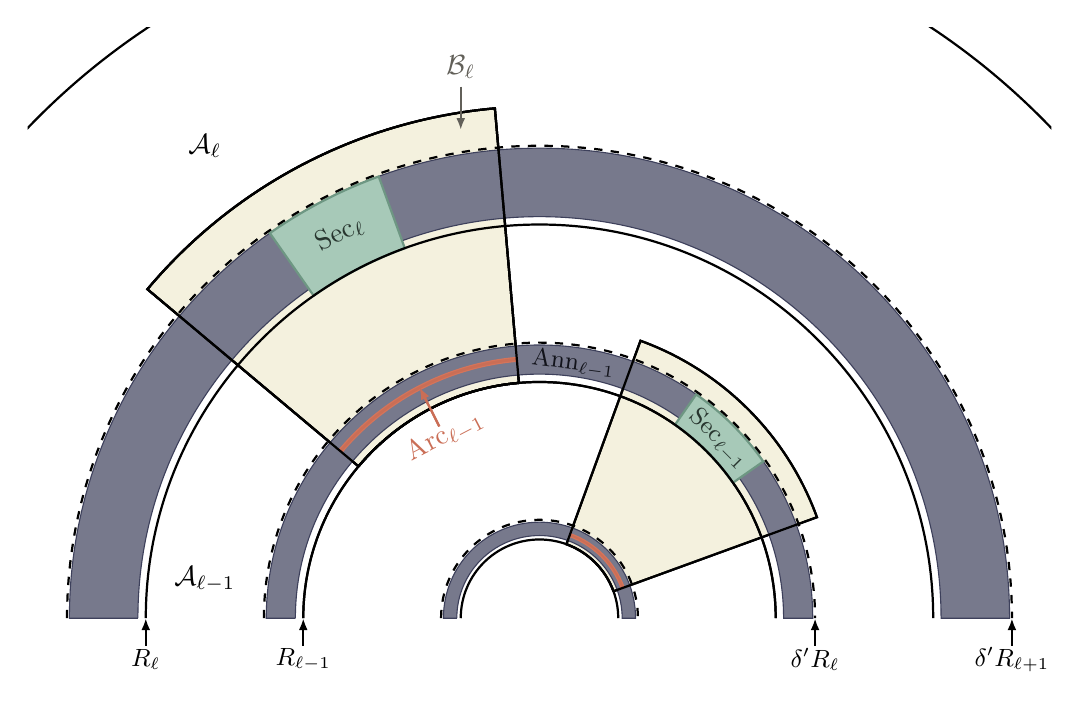
\begin{tikzpicture}

\clip(-1.5,-1) rectangle (11.5,7.5);

\begin{scope}[shift={(5,0)}]
\draw[thick] (180:9) arc (180:0:9);
\end{scope}



\begin{scope}[shift={(5,0)}]
\draw[thick,fill=tan1] (20:1) -- (20:3.75) arc (20:70:3.75) -- (70:1) arc (70:20:1);
\end{scope}

\begin{scope}[shift={(5,0)},rotate=10]
\draw[thick,fill=tan1] (130:3) -- (130:6.5) arc (130:85:6.5) -- (85:3) arc (85:130:3);
\end{scope}

\begin{scope}[shift={(5,0)}]
\draw[color=blue1,fill=blue1!70] (180:5.1) -- (180:5.97) arc (180:0:5.97) -- (0:5.1) arc (0:180:5.1);
\end{scope}


\begin{scope}[shift={(5,0)},rotate=10]

\draw[thick] (130:3) -- (130:6.5) arc (130:85:6.5) -- (85:3) arc (85:130:3);
\draw[thick, color=green1!85!black,fill=green1!70] (115:5) -- (115:5.97) arc (115:100:5.97) -- (100:5) arc (100:115:5);
\node[rotate=17.5+10,color=green1!30!black] at (-1.65,5.25) {$\mathrm{Sec}_\ell$};
\end{scope}


\node at (0.75,6) {$\A_\ell$};
\node at (0.75,0.5) {$\A_{\ell-1}$};
\draw[thick,dashed] (-1,0) arc (180:0:6);



\begin{scope}[shift={(5,0)}]
\draw[color=blue1,fill=blue1!70] (180:3.1) -- (180:3.47) arc (180:0:3.47) -- (0:3.1) arc (0:180:3.1);
\node[rotate=-7.5,color=blue1!30!black] at (0.43,3.23) {\small $\mathrm{Ann}_{\ell-1}$};
\end{scope}

\draw[thick] (2,0) arc (180:0:3);
\begin{scope}[shift={(5,0)},rotate=10]
\draw[color=red1!95!black,fill=red1!90!black] (130:3.3-0.025) -- (130:3.3+0.025) arc (130:85:3.3+0.025) -- (85:3.3-0.025) arc (85:130:3.3-0.025);
\node[color=red1!90!black,rotate=27.5] at (-0.78,2.48) {$\mathrm{Arc_{\ell-1}}$};
\draw[color=red1!90!black,thick,-{Latex[length=1.5mm]}] (-0.83,2.62) -- (-0.99,3.15);
\end{scope}

\begin{scope}[shift={(5,0)},rotate=10]
\draw[thick] (130:3) -- (130:6.5) arc (130:85:6.5) -- (85:3) arc (85:130:3);
\end{scope}


\begin{scope}[shift={(5,0)}]
\draw[color=blue1,fill=blue1!70] (180:1.05) -- (180:1.22) arc (180:0:1.22) -- (0:1.05) arc (0:180:1.05);
\draw[color=red1!95!black,fill=red1!90!black] (20:1.125--0.02) -- (20:1.125+0.02) arc (20:70:1.125+0.02) -- (70:1.125-0.02) arc (70:20:1.125-0.02);
\end{scope}


\begin{scope}[shift={(5,0)}]
\draw[thick] (20:1) -- (20:3.75) arc (20:70:3.75) -- (70:1) arc (70:20:1);
\draw[thick,color=green1!85!black,fill=green1!70] (40-5:3) -- (40-5:3.47) arc (40-5:50+5:3.47) -- (50+5:3) arc (50+5:40-5:3);
\node[rotate=-45,color=green1!30!black] at (2.27,2.27) { \small $\mathrm{Sec}_{\ell-1}$};
\end{scope}

\draw[thick] (2,0) arc (180:0:3);

\begin{scope}[shift={(5,0)},rotate=10]
\draw[color=red1!90!black,thick,-{Latex[length=1.5mm]}] (-0.83,2.62) -- (-0.99,3.15);
\end{scope}

\draw[thick,dashed] (1.5,0) arc (180:0:3.5);
\draw[thick] (0,0) arc (180:0:5);

\node[fill=white] at (2,-0.525) {\small $R_{\ell-1}$};
\draw[thick,-{Latex[length=1.5mm]}] (2,-0.35) -- (2,0);

\node at (8.5,-0.525) {\small $\delta' R_{\ell}$};
\draw[thick,-{Latex[length=1.5mm]}] (8.5,-0.35) -- (8.5,0);

\node at (0,-0.525) {\small $R_{\ell}$};
\draw[thick,-{Latex[length=1.5mm]}] (0,-0.35) -- (0,0);

\node at (11,-0.525) {\small $\delta' R_{\ell+1}$};
\draw[thick,-{Latex[length=1.5mm]}] (11,-0.35) -- (11,0);

\node[color=tan1!40!black] at (4,7) {$\mathcal{B}_{\ell}$};
\draw[thick,color=tan1!40!black,-{Latex[length=1.5mm]}] (4,6.75) -- (4,6.2);

\draw[thick] (4,0) arc (180:0:1);
\draw[thick,dashed] (3.75,0) arc (180:0:1.25);

\end{tikzpicture}


\end{document}